\chapter{คู่มือการใช้งานแอปพลิเคชันค้นหายาเพื่อคุณ}
คู่มือการใช้งานแอปพลิเคชันค้นหายาเพื่อคุณ 
มีวิธีการใช้งานดังต่อไปนี้ 
เมื่อผู้ใช้งานเปิดแอปพลิเคชันจะพบกับหน้าแรก 
ดังแสดงในภาพที่ ค.1 
และหลังจากแสดงหน้าแรก 1.5 วินาที 
ระบบเปลี่ยนไปแสดงหน้าค้นยา 
ดังแสดงในภาพที่ ค.2

\begin{figure}[H]
    \centering
\includegraphics[scale=1.2]{Figures/7/14}
    \caption{หน้าแรกของแอปพลิเคชันค้นหายาเพื่อคุณ}
    \label{Fig:howto1}
\end{figure}


\begin{figure}[H]
    \centering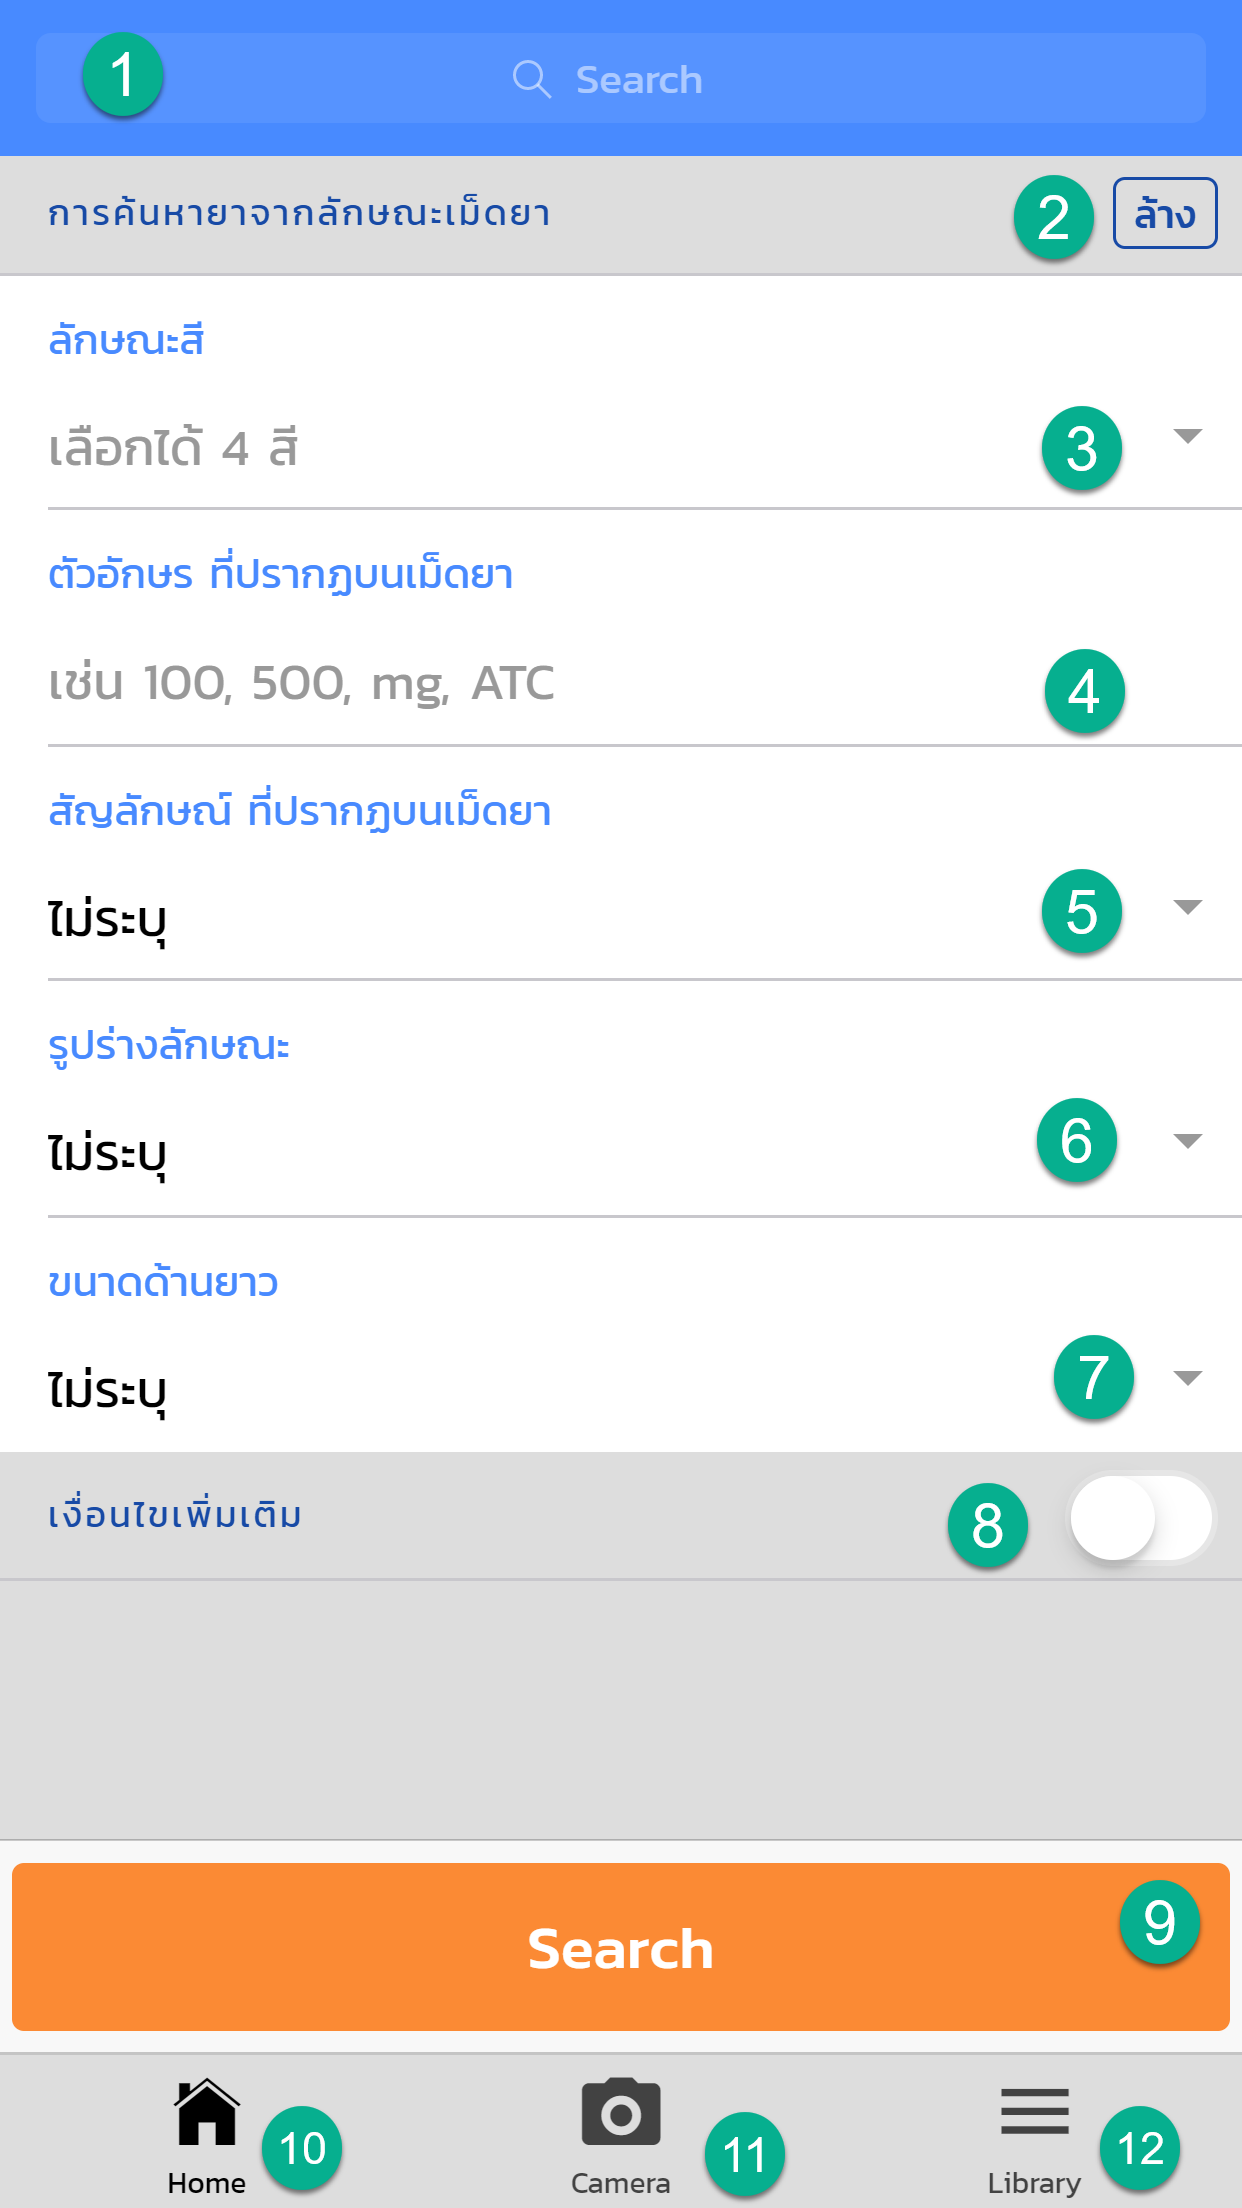
\includegraphics[scale=0.2]{Figures/7/15}
    \caption{หน้าค้นหายาของแอปพลิเคชันค้นหายาเพื่อคุณ}
    \label{Fig:howto2}
\end{figure}

จากภาพที่ \ref{Fig:howto2} หน้าการค้นหายา เป็นหน้าสำหรับค้นหายาโดยใส่ข้อมูลลักษณะของยาลงไปในช่องกรอกข้อมูล และสามารถอธิบายรายละเอียดต่างๆของหน้าค้นหายาได้ดังนี้
\begin{itemize}[label={--}]
	\item หมายเลข 1 คือ ช่องกรอกคำค้นหาแบบทั่วไป สามารถกรอกข้อมูลคำคัญได้
    \item หมายเลข 2 คือ สามารถกดเพื่อล้างคำค้นหาในหน้าค้นหายาได้ 
    \item หมายเลข 3 คือ สามารถกดเพื่อเลือกลักษณะสีของยาได้มากสุด 4 สี
    \item หมายเลข 4 คือ ช่องกรอกข้อมูลตัวอักษณะที่ปรากกฏบนเม็ดยา
    \item หมายเลข 5 คือ สามารถกดเพื่อเลือกสัญลักษณ์ที่ปรากฏบนเม็ดยาได้
    \item หมายเลข 6 คือ สามารถกดเพื่อเลือกรูปร่างลักษณะของเม็ดยาได้
    \item หมายเลข 7 คือ สามารถกดเพื่อเลือกขนาดด้านยาวของเม็ดยาได้
    \item หมายเลข 8 คือ สามารถกดเพื่อแสดงเงื่อนไขเติมของการค้นหายาจากลักษณะเม็ดได้
    \item หมายเลข 9 คือ สามารถกดเพื่อค้นหาจากการนำข้อมูลหมายเลข 3-7 ไปค้นหา และจะแสดงไปยังหน้ารายการค้นหา
    \item หมายเลข 10 คือ สามารถกดเพื่อไปยังหน้าค้นหา (Home) 	 
    \item หมายเลข 11 คือ สามารถกดเพื่อไปยังหน้ากล้องถ่ายรูป
    \item หมายเลข 12 คือ สามารถกดเพื่อไปยังหน้าไลบรารี่
\end{itemize}

\begin{figure}[H]
    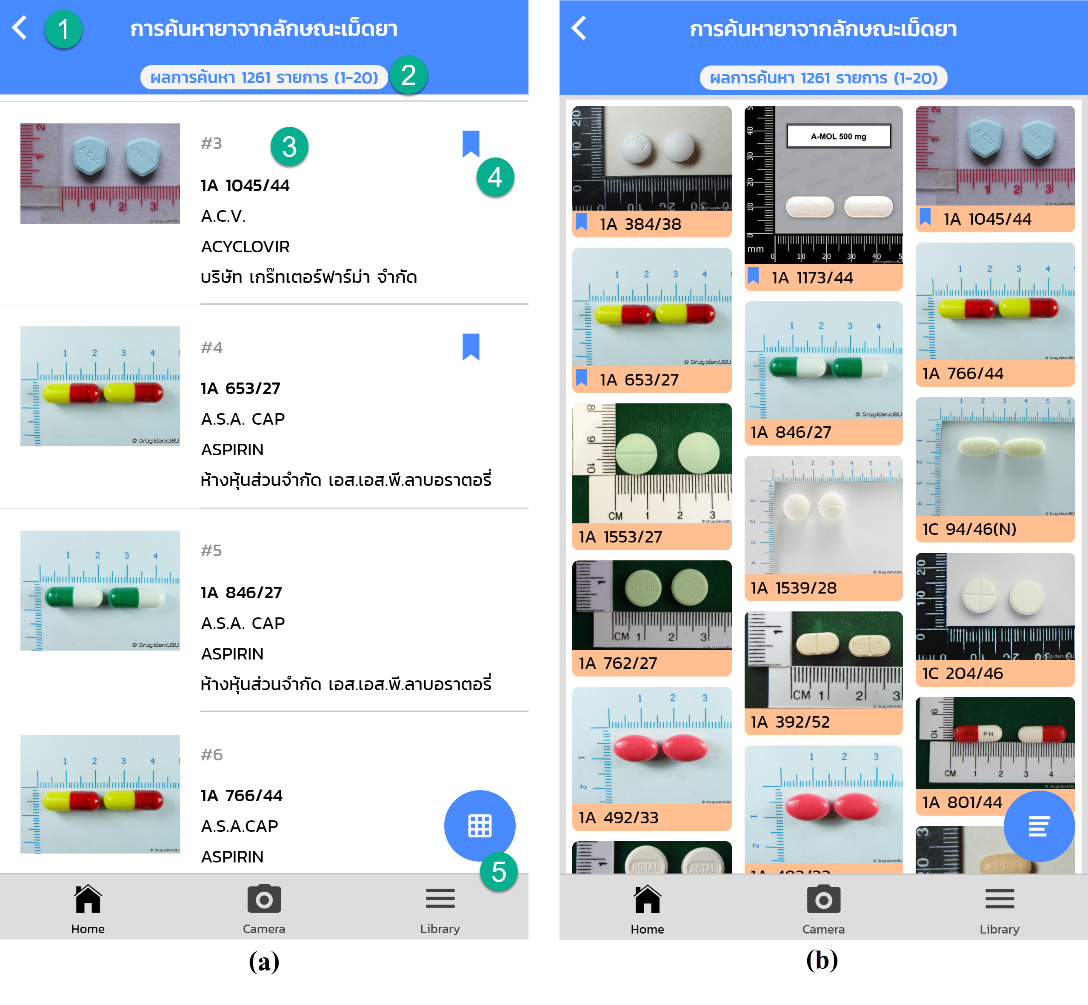
\includegraphics[width=\columnwidth]{Figures/7/16}
    \caption{หน้ารายการการค้นหายา}
    \label{Fig:howto3}
\end{figure}

จากภาพที่ \ref{Fig:howto3} หน้ารายการการค้นหายาแบบรายการ เมื่อผู้ใช้งานกดค้นหาหรือกรอกคำค้นหาแบบทั่วไปในช่องค้นหา แอปพลิเคชันจะแสดงหน้ารายการค้นหายา ผู้ใช้งานสามารถเลื่อนขึ้นและเลื่อนลงเพื่อดูรายการค้นหายาได้ ถ้าหากผู้ใช้กดเลือกรายการยา แอปพลิเคชันจะแสดงหน้ารายละเอียดเม็ดยาที่ผู้ใช้งานกดเลือก อธิบายรายละเอียดดังนี้
\begin{itemize}[label={--}]
	\item หมายเลข 1 คือ สามารถกดย้อนกลับไปหน้าค้นหาได้
    \item หมายเลข 2 คือ แสดงจำนวนรายการที่ค้นหาเจอทั้งหมด
    \item หมายเลข 3 คือ แสดงเลขลำดับของรายการยา และสามารถกดแตะเพื่อดูรายละเอียดของรายการยาได้
    \item หมายเลข 4 คือ เครื่องหมายบุ๊กมาร์ก ถ้าหากรายการยามีเครื่องหมายบุ๊กมาร์กติดอยู่ หมายความว่า รายการยาถูกบุ๊กมาร์กไว้แล้วในเครื่องผู้ใช้งาน
    \item หมายเลข 5 คือ สามารถกดเพื่อเปลี่ยนรูปแบบการแสดงรายการยาจากรายการเป็นรูปขนาดย่อ  (Thumbnails) ได้ ดังภาพที่ ค.3 (b)
\end{itemize}

\begin{figure}[H]
    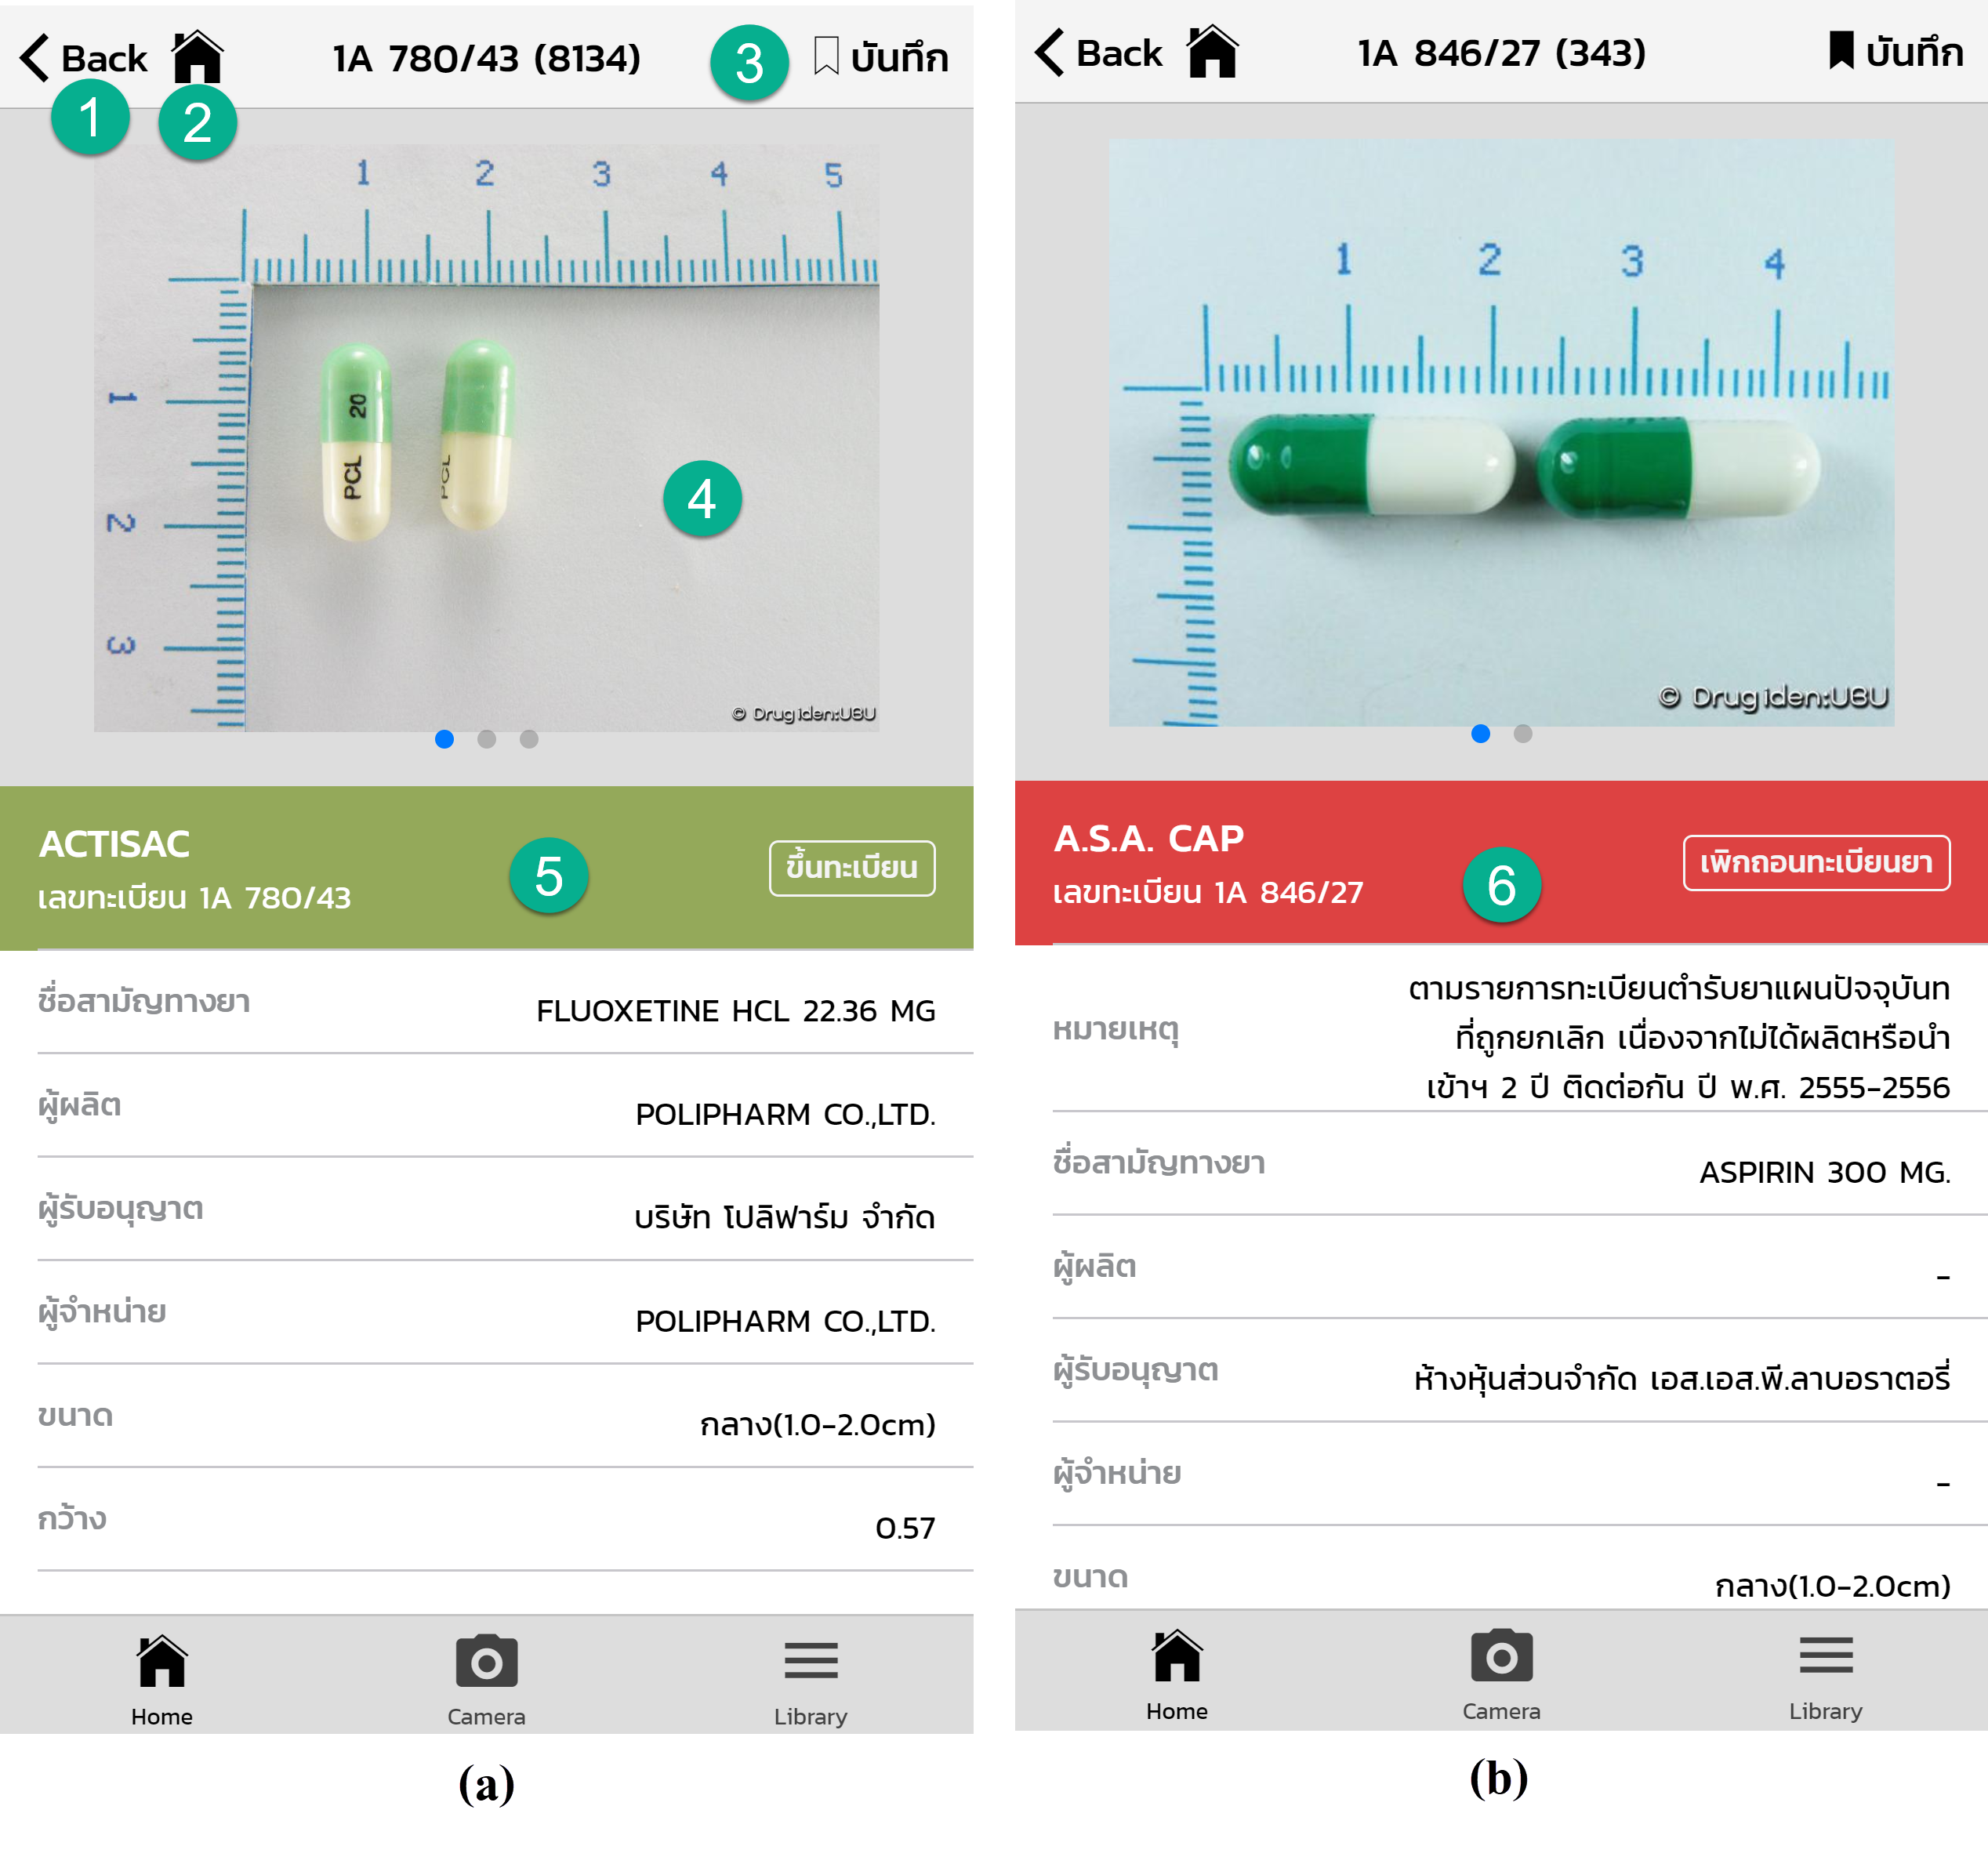
\includegraphics[width=\columnwidth]{Figures/7/17}
    \caption{หน้าแสดงรายละเอียดยา}
    \label{Fig:howto4}
\end{figure}

จากภาพที่ \ref{Fig:howto4} หน้าแสดงรายละเอียดยา เมื่อผู้ใช้งานกดเลือกรายการยาจากหน้ารายการยา แอปพลิเคชันจะแสดงหน้ารายละเอียด อธิบายรายละเอียดดังนี้
\begin{itemize}[label={--}]
	\item หมายเลข 1 คือ สามารถกดเพื่อย้อนกลับไปยังหน้าแสดงรายการการค้นหายาได้
    \item หมายเลข 2 คือ สามารถกดเพื่อกลับไปยังหน้าค้นหายาได้
    \item หมายเลข 3 คือ สามารถกดบันทึกบุ๊กมาร์กได้ ถ้าหากสัญลักษณ์บุ๊กมาร์กเป็นดังภาพที่ ค.4 (a) หมายถึงรายการยายังไม่ได้ถูกบุ๊กมาร์ก
    \item หมายเลข 4 คือ สามารถกดที่รูปภาพเพื่อขยายรูปภาพให้ใหญ่ขึ้นได้
    \item หมายเลข 5 คือ แสดงชื่อสามัญของเม็ดยา เลขทะเบียน และถ้ามีบราเป็นสีเขียวหมายถึงสถานะของยาขึ้นอยู่เทียน
    \item หมายเลข 6 คือ แสดงชื่อสามัญของเม็ดยา เลขทะเบียน และถ้ามีบราเป็นสีแดงหมายถึงสถานะของถูกเพิกถอนไปแล้ว และสามารถดูรายละเอียดที่หมายเหตุได้
\end{itemize}

\begin{figure}[H]
    \centering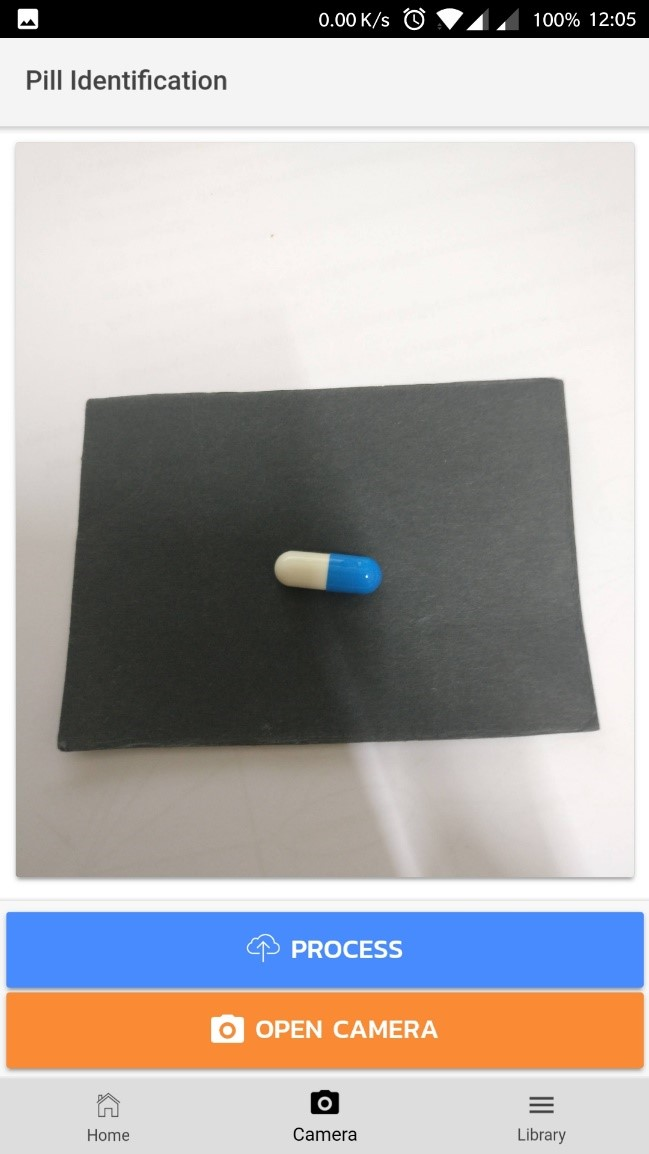
\includegraphics[scale=0.9]{Figures/7/18}
    \caption{หน้าถ่ายรูปภาพ}
    \label{Fig:howto5}
\end{figure}

จากภาพที่ \ref{Fig:howto5} หน้าถ่ายรูปภาพ 
เป็นหน้าสำหรับการถ่ายรูปภาพเม็ดยาเพื่อพิสูจน์เอกลักษณ์ยา 
โดยนำเม็ดยาวางไว้บนวัถตุอ้างอิงสีดำที่มีขนาดด้านยาว 10 เซนติเมตร ด้านกว้าง 7 เซนติเมตร 
และใช้กล้องถ่ายรูปถ่ายรูปจากมุมสูง เมื่อถ่ายรูปภาพเสร็จแล้ว 
แอปพลิเคชันจะแสดงดังภาพที่ \ref{Fig:howto5} (a)

เมื่อผู้ใช้งานกดประมวลผล (Process) แอปพลิเคชันจะแสดงผลลัพธ์การพิสูจน์เอกลักษณ์ยาเม็ดที่หน้าแสดงผลลัพธ์การพิสูจน์เอกลักษณ์ยา
ดังภาพที่ \ref{Fig:howto5} (b) 
และยังสามารถแก้ไขผลลัพธ์เพื่อใช้ค้นหายาได้ด้วยการกดค้นหาเพื่อดูรายการค้นหาที่แก้ไขไปได้

\begin{figure}[H]
    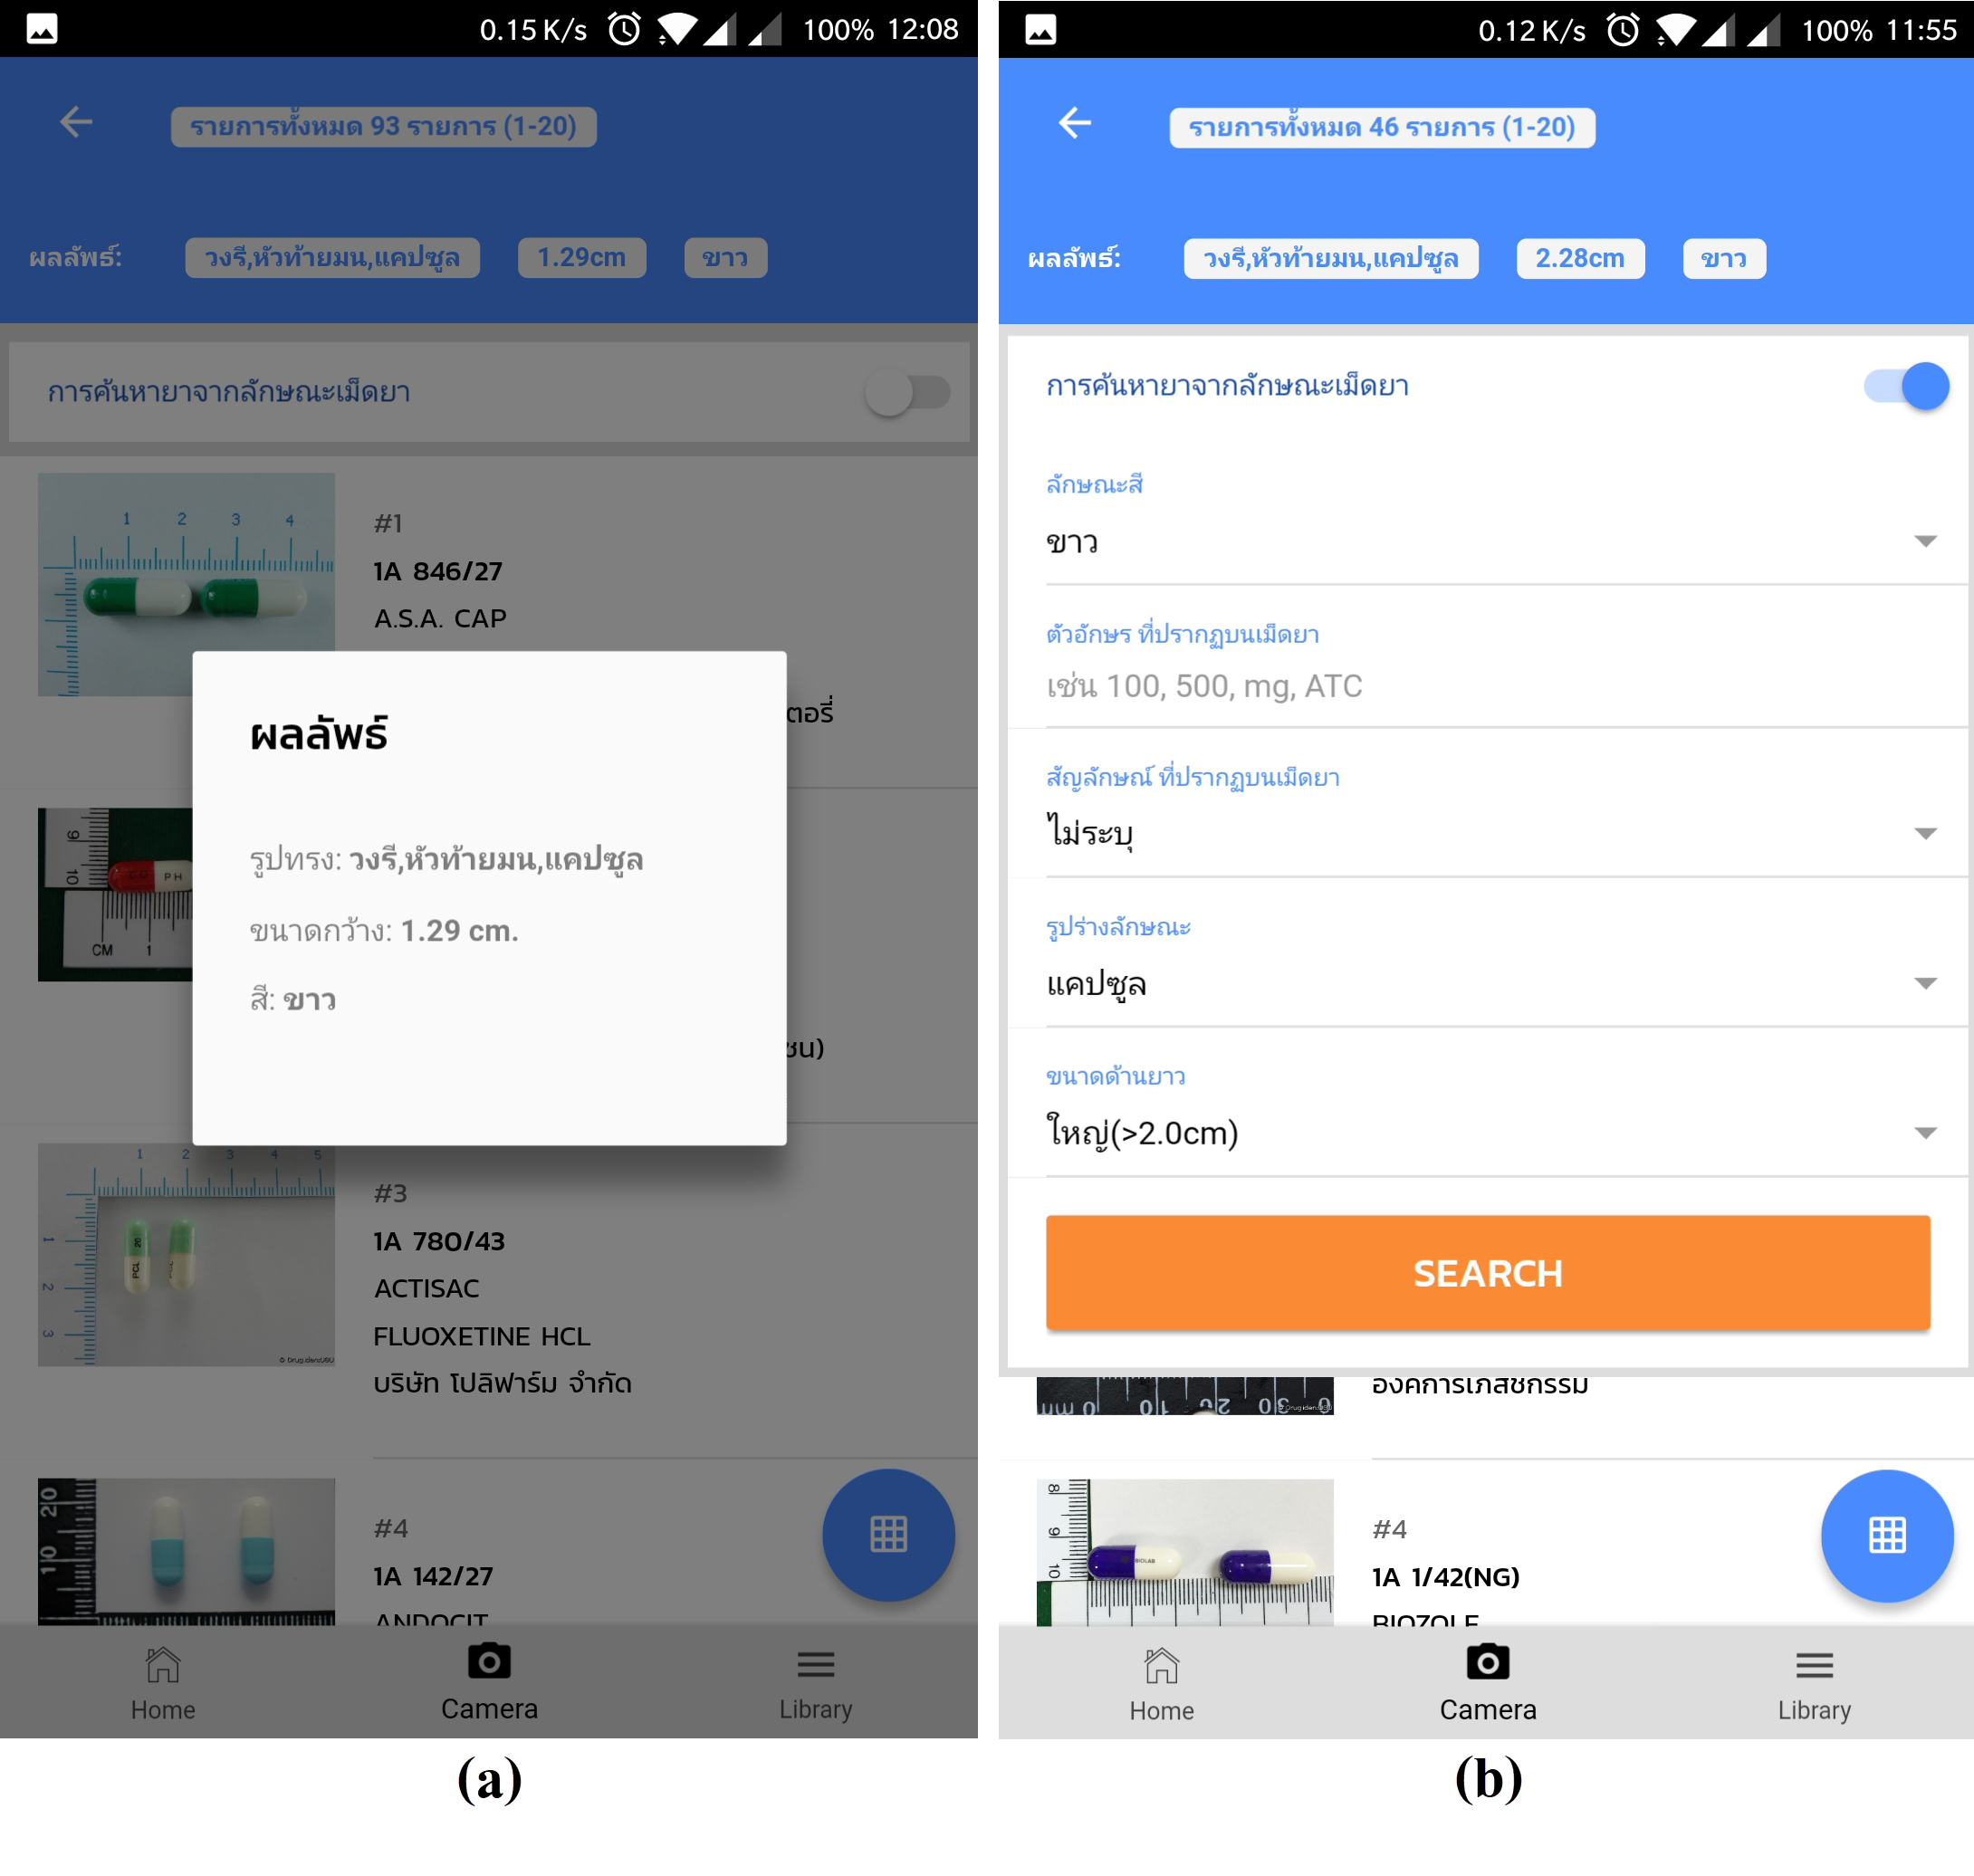
\includegraphics[width=\columnwidth]{Figures/7/19}
    \caption{หน้าแสดงผลลัพธ์การพิสูจน์เอกลักษณ์ยา}
    \label{Fig:howto6}
\end{figure}

